%%% LaTeX Template: Two column article
%%%
%%% Source: http://www.howtotex.com/
%%% Feel free to distribute this template, but please keep to referal to http://www.howtotex.com/ here.
%%% Date: February 2011

%%% Preamble
\documentclass[	DIV=calc,%
							paper=a4,%
							fontsize=12pt,%
							onecolumn]{scrartcl}	 					% KOMA-article class

\usepackage{lipsum}													% Package to create dummy text
\usepackage[brazil]{babel}										% English language/hyphenation
\usepackage[protrusion=true,expansion=true]{microtype}				% Better typography
\usepackage{amsmath,amsfonts,amsthm}					% Math packages
\usepackage[pdftex]{graphicx}									% Enable pdflatex
\usepackage[svgnames]{xcolor}									% Enabling colors by their 'svgnames'
\usepackage[hang, small,labelfont=bf,up,textfont=it,up]{caption}	% Custom captions under/above floats
\usepackage{epstopdf}												% Converts .eps to .pdf
\usepackage{subfig}													% Subfigures
\usepackage{booktabs}												% Nicer tables
\usepackage{fix-cm}													% Custom fontsizes
\usepackage[utf8]{inputenc}
\usepackage[top=2.5cm, bottom=2.5cm, left=2.5cm, right=2.5cm]{geometry}
\usepackage[ddmmyyyy]{datetime}
\usepackage{indentfirst}
\addto\captionsenglish{%
	\renewcommand\tablename{Tabela}
	\renewcommand\figurename{Figura}
} 
 

 
%%% Custom sectioning (sectsty package)
\usepackage{sectsty}													% Custom sectioning (see below)
\allsectionsfont{%															% Change font of al section commands
	\usefont{OT1}{phv}{b}{n}%										% bch-b-n: CharterBT-Bold font
	}

\sectionfont{%																% Change font of \section command
	\usefont{OT1}{phv}{b}{n}%										% bch-b-n: CharterBT-Bold font
	}



%%% Headers and footers
\usepackage{fancyhdr}												% Needed to define custom headers/footers
	\pagestyle{fancy}														% Enabling the custom headers/footers
\usepackage{lastpage}	

% Header (empty)
\lhead{}
\chead{}
\rhead{}
% Footer (you may change this to your own needs)

%% ====================================
%% ====================================
%% mude o rodape  do projeto
%% ====================================
%% ====================================

\lfoot{\footnotesize \texttt{Template de documento para processo de software} \textbullet ~Modelo BJR}


\cfoot{}
\rfoot{\footnotesize página \thepage\ de \pageref{LastPage}}	% "Page 1 of 2"
\renewcommand{\headrulewidth}{0.0pt}
\renewcommand{\footrulewidth}{0.4pt}



%%% Creating an initial of the very first character of the content
\usepackage{lettrine}
\newcommand{\initial}[1]{%
     \lettrine[lines=3,lhang=0.3,nindent=0em]{
     				\color{DarkGoldenrod}
     				{\textsf{#1}}}{}}



%%% Title, author and date metadata
\usepackage{titling}															% For custom titles

\newcommand{\HorRule}{\color{DarkGoldenrod}%			% Creating a horizontal rule
									  	\rule{\linewidth}{1pt}%
										}

\pretitle{\vspace{-30pt} \begin{flushleft} \HorRule 
				\fontsize{50}{50} \usefont{OT1}{phv}{b}{n} \color{DarkRed} \selectfont 
				}

%% ====================================
%% ====================================
%% mude o titulo  do projeto
%% ====================================
%% ====================================

\title{Modelo de Processo BJR}					% Title of your article goes here

%% ====================================



\posttitle{\par\end{flushleft}\vskip 0.5em}

\preauthor{\begin{flushleft}
					\large \lineskip 0.5em \usefont{OT1}{phv}{b}{sl} \color{DarkRed}}
\author{Breno Angelotti, Gabriel Romero, Jean Gonçalves, João Goulart, Mateus Merscher, Renan Batel }  	% Author name goes here


\postauthor{\footnotesize \usefont{OT1}{phv}{m}{sl} \color{Black} 
					\\Universidade Tecnológica Federal do Paraná - Câmpus Cornélio Procópio 								% Institution of author
					\par\end{flushleft}\HorRule}

\date{}																				% No date




%%% Begin document
\begin{document}
\maketitle
\thispagestyle{fancy} 	
\thispagestyle{empty}		% Enabling the custom headers/footers for the first page 
% The first character should be within \initial{}




%% ====================================
%% ====================================
%% mude o resumo  do projeto
%% ====================================
%% ====================================
\initial{E}\textbf{ste modelo de processo de software apresenta uma metologia de desenvolvimento ágil e cíclico para pequenos times de desenvolvimento com foco em projetos SaaS.}

%% ====================================
\begin{figure}
	\centering
	
\includegraphics{utfpr}
\end{figure}

\vspace{3cm}
\centerline{\textit{\textbf{\today}}}

\clearpage
    \renewcommand*\listfigurename{Lista de figuras}
\listoffigures


\clearpage
\renewcommand{\contentsname}{Sumário}
\tableofcontents
\clearpage

%% ====================================
%% ====================================
%% Inicio do texto
%% ====================================
%% ====================================
\section{Introdução}
O modelo de processo de software apresentado neste documento é de estrutura ágil para equipes pequenas com projetos de empresas que tenham Software as a Service (SaaS)\cite{saas}. A proposta desse modelo é a autonomia do time de desenvolvimento e a visibilidade que cada desenvolvedor tem dentro do projeto, tudo isso contido dentro de um ciclo de desenvolvimento rápido e eficaz.

\begin{itemize}
	\item Modelo de Processo Ágil BJR;
	\item Integrantes: Breno Angelotti; Gabriel Romero; Jean Carlos Gonçalves; João Victor Goulart de Almeida; Mateus Merscher; Renan Batel.
	\item Github: https://github.com/goulartt/template;
\end{itemize}


\section{Processo}
O modelo de processo de software desenvolvido é de categoria ágil com ciclo de vida cíclico. O foco desse processo é desenvolver de forma rápida, e dando autonomia para equipe de desenvolvimento, ideal para empresas que contenham SaaS e várias equipes pequenas (squads) \cite{spotify}  de desenvolvimento.

\subsection{Fases}
	\subsubsection{Levantamento de Requisitos}
	A fase inicial deste processo é a fase de Levantamento de Requisitos, onde é realizada a comunicação com o cliente. Essa comunicação é de extrema importância, sendo realizada através de reuniões onde serão estabelecidos parâmetros para toda a parte de planejamento, nestas reuniões devem ser levantados os requisitos do cliente e os objetivos que a entrega deve atingir, quanto mais informações forem obtidas mais claros ficarão os objetivos. 
	
	Ainda na fase de Levantamento de Requisitos ocorre o planejamento das fases seguintes com base no que foi levantado com o cliente, durante o planejamento deve ficar claro quais serão as prioridades para que se possa agregar valor à entrega, uma boa execução desta fase facilitará o fluxo das outras. 
	
	\subsubsection{Desenvolvimento}
	Finalizada a fase inicial do processo, os artefatos necessários para a construção do projeto já estão formalizados, sendo assim a próxima fase trata do Desenvolvimento. 
	
	A fase de Desenvolvimento começa com uma discussão sobre os itens que deverão ser produzidos. Durante essa fase são definidos quais itens serão feitos e qual será a ordem de execução baseado nas prioridades do cliente. Assim que os itens são definidos começa-se a produção dos mesmos. 
	
	\subsubsection{Análise e Teste}
	 Após o término do Desenvolvimento, os itens produzidos devem ser testados, nesse momento temos a fase de Análise e Teste. Nesta etapa o time é responsável por verificar se o conteúdo gerado a partir da fase anterior possui erros ou pendências técnicas. 
	
	 Quando o fluxo não apresenta erros ou falhas, é necessário validar se o conteúdo cumpre aquilo especificado no planejamento, podemos dizer que essa fase verifica de modo detalhado se os itens estão preparados para a fase seguinte ou não. 
	
	\subsubsection{Entrega}
	A próxima etapa, de Entrega, depende fortemente de suas antecessoras, pois para que toda as suas tarefas sejam feitas, a especificação deve ter sido clara, a implementação deve ter ocorrido, e todos os itens devem ter sido validados e testados, nesta fase é registrado como os itens foram construídos e também o que realmente foi produzido nas duas fases anteriores. 
	
	Também é nesta fase onde ocorre o versionamento dos artefatos gerados, a versão considerada estável do produto é implantada no ambiente de produção e, para finalizar, o resultado do acompanhamento de todo o ciclo é apresentado para a equipe. 
	
	\subsubsection{Manutenção}
	Ao final do nosso ciclo do processo temos a fase de Manutenção, nesta fase o time se preocupa em manter o funcionamento do sistema, nela é de grande importância o monitoramento do produto para a geração de relatórios, com foco especial nos itens do último pacote entregue, o relatório auxiliará mais tarde na priorização e construção de correções. 

\subsection{Papéis}
O ideal para utilização desse modelo é uma equipe de 5 a 7 pessoas, sendo que toda equipe deve conter um Customer (cliente), um Agile Coach, um Product Owner, uma equipe de desenvolvimento e um Line Manager (Opcional), cuja suas respectivas funções são: 
\begin{itemize}
	\item \textbf{Customer}: O cliente tem o papel principal para o processo ocorrer, ele será o responsável por ditar o produto/serviço que será desenvolvido.
	\item \textbf{Agile Coach}: Ajuda a manter o fluxo de trabalho, facilitando as retrospectivas, as reuniões de planejamento do ciclo, organizar a equipe de desenvolvimento e garantir a entrega prevista do ciclo. 
	
	\item \textbf{Product Owner}:\cite{scrumguide} Responsável pelo backlog e define prioridades das histórias, se comunicando diretamente com os stakeholders e apresentar ao cliente o andar do desenvolvimento do software. 
	
	\item \textbf{Squad}: Equipe de desenvolvimento, quem vai codificar a solução.
	
	\item \textbf{Line Manager}: responsável por no máximo 5 squads, irá alinhar com as equipes o que está sendo feito, participará em algumas reuniões para acompanhamento do squad sem influenciar no processo. Responsável pelo coaching e desenvolvimento de carreira individual de cada membro dos squads. Acompanha reclamações e problemas para criar planos de ação que melhorem o processo. 
\end{itemize}

\subsection{Tarefas}
Este processo de desenvolvimento não é orientado a atividades, e sim a tarefas diretamente, como se trata de um processo ágil com um ciclo de vida cíclico e de duração indeterminada, os deadlines de cada tarefa é definido por quem o aplica, entretanto, para um melhor aproveitamento do processo, é aconselhável que o deadline das tarefas de planejamento(Especificação de requisitos, Construção da história e Definição de backlogs e prioridades) não ultrapasse  o início tarefa de Planejamento do Desenvolvimento, já as demais tarefas, o deadline sugerido é fase de Entrega. 
As definições de cada tarefa e seus papeis relacionados se encontram logo abaixo: 
\begin{itemize}
	\item \textbf{Especificação de requisitos}: Durante uma reunião entre o Product Owner e o Customer para estabelecer os requisitos do cliente, o Product Owner deverá extrair o máximo de informações possíveis do Customer, após essa reunião o Product Owner deve analisar o que foi obtido e identificar os requisitos do projeto, quanto mais informações forem obtidas mais fácil será identificar os requisitos do projeto para satisfazer os requisitos do cliente;  
	
	\item \textbf{Construção da história}: O Product Owner construirá as histórias, com base nos requisitos já levantados por ele, as Histórias servirão para esclarecer melhor os requisitos e as funcionalidades, elas devem ser simples, curtas e claras, devem ser feitas utilizando do ponto de vista de um usuário;
	
	\item \textbf{Definição de backlogs e prioridades}: O Product Owner deve montar o backlog com o que será feito e definir as prioridades de cada um dos itens com base nas prioridades do cliente; 
	
	\item \textbf{Manter fluxo}: Durante o caminhar do projeto o Agile Coach deve ajudar a manter o fluxo de execução das fases e tarefas seguindo como o planejado e ajudar na comunicação entre as equipes de desenvolvimento; 
	
	\item \textbf{Planejamento de Desenvolvimento}:  Em uma reunião o Squad junto do Agile Coach definirão os itens que a serem desenvolvidos durante este ciclo do projeto e a duração do ciclo com base nas estimativas de tempo levantadas pelo Squad para cada item, 20\% do tempo estimado será dedicado aos testes e correções e 10\% do tempo estimado deve ser definido como respiro; 
	
	\item \textbf{Implementação da Sprint}: Os itens definidos na tarefa de Planejamento de Desenvolvimento devem ser desenvolvidos pelo Squad dentro do tempo que foi planejado;  
	
	\item \textbf{Correções}: O Squad responsável realizará as correções que forem identificadas durante o desenvolvimento ou durante os testes no tempo dedicado a correções definido no Planejamento de Desenvolvimento; 
	
	\item \textbf{Criação dos casos de teste}: : os casos de testes são especificados pelo Squad a partir das funções desenvolvidas, as especificações incluem testes unitários e testes de integrações entre as funções, os casos devem ser registrados de forma rastreável aos requisitos;
	
	\item \textbf{Construção dos testes}: À partir da especificação dos casos de teste, o Squad deve realizar a construção dos scripts de teste; 
	
	\item \textbf{Execução dos testes}:  Após a criação dos testes os mesmos deverão ser executados pelo Squad no produto nos diferentes ambientes necessários, e caso encontrado algum comportamento diferente do esperado, é necessário rastrear a causa e realizar a correção; 
	
	\item \textbf{Validação}: O Squad analisa os resultados dos testes e das correções e o pacote funcional é liberado para entrega, caso ainda haja falhas elas não devem estar incluídas no pacote a ser entregue; 
	
	\item \textbf{Documentação dos artefatos}: Todos os artefatos são registrados (P.O, Agile Coach, Squad); 
	
	\item \textbf{Versionamento}: Os artefatos são versionados (P.O, Agile Coach, Squad); 
	
	\item \textbf{Implantação}: Após todas as validações um pacote sem falhas e estável é enviado para produção pelo Squad;
	
	\item \textbf{Análise e priorização da manutenção}:  o Agile Coach junto com o Squad é responsável pela análise do relatório de erros coletados do sistema, o Agile Coach analisa as incidências e número de usuários afetados para apontar a relevância do erro, o Squad deve discutir o nível de dificuldade para e qual o impacto da implementação da correção, feito isso, os números são analisados e as ações/correções são priorizadas; 
	
	\item \textbf{Análise e priorização da manutenção}: o Agile Coach deve realizar uma nova análise sobre as ações/correções priorizadas e definir quando as mesmas serão implementadas. 
\end{itemize}

\subsection{Disciplinas}
O componente de disciplina se aplica ao conjunto de atividades relacionadas, as quais podemos associar:
\begin{itemize}
		\item \textbf{Desenvolvimento:} Implementação da Sprint, Correções, Versionamento, Implantação; 
		\item \textbf{Teste de Software:} Criação dos casos de teste, Construção dos testes, Execução dos testes; 
		\item \textbf{Sustentação:}  Planejamento da Manutenção, Feedback, Análise e priorização da manutenção; 
		\item \textbf{Gestão de Projetos:}  Feedback, Manter Fluxo, Planejamento de Sprint, Validação, Documentação, Versionamento; 
		\item \textbf{Análise de Requisitos:} Especificação de requisitos, Construção da História, Definição de Backlog e priorização, Validação; 
\end{itemize}	


\subsection{Artefatos}
Os artefatos gerados durante o processo são de sua maioria relatórios para coleção e análise de dados, que são:
\begin{itemize}
	\item \textbf{Relatório negativo do ciclo:} Nesse relatório será coletado dificuldades presentes, erros que ocorreram no ciclo, atrasos e qualquer indicador negativo presente no ciclo.
	\item \textbf{Relatório positivo do ciclo:} É coletado tudo que ocorreu com sucesso, evidências que fizeram isso ocorrer para poder ser analisado e repetir nos próximos ciclos. 
	\item \textbf{Relatório Quantitativo:} Indicadores tais como porcentagem de funcionalidades entregues, pontos por estimativa daquele ciclo, erros introduzidos por ciclo e ranqueamento das causas.
\end{itemize}

E para finalizar podemos citar como artefato a versão nova do sistema desenvolvido, a cada entrega que for feita será alterado a versão do sistema e versionada.
\subsection{Guidance}
\subsubsection{Guidlines} 
\paragraph{Material Design}
Utilizado para definir a componentização e padronização dos elementos visuais, o Material Design\cite{materiald} tem como principal característica o uso de metáforas visuais que auxiliam no reconhecimento do comportamento do sistema e aumentam a facilidade de uso do sistema. Toda a componentização se baseia em como se comportam materiais reais, como folhas sobrepostas, por exemplo.

\paragraph{SOLID Principles}
Os princípios SOLID\cite{solid} é um conjunto de ideais a serem seguidos em um projeto de software com desenvolvimento orientado a objetos com o objetivo de gerar um software com maior qualidade, alta manutenibilidade e facilidade para testes. Estes princípios são:
\begin{itemize}
	\item \textbf{Single responsibility principle (SRP):} ou princípio de responsabilidade única, define que uma classe deve ter apenas uma funcionalidade como sua responsabilidade. Ex: uma classe de acesso à API não deve trabalhar seus dados de resposta, apenas comunicar-se com o serviço e repassar os dados para a classe que chamou o método;
	\item \textbf{Open/closed principle (OCP):} o princípio aberto-fechado define que uma classe possa ter seu comportamento estendido sem que sua estrutura seja alterada, ou seja, aberto para extensão, mas fechado para modificação;
	\item \textbf{Liskov substitution principle (LSP):} de acordo com o princípio de substituição de Liskov, deve ser possível substituir um objeto por outro de seu subtipo sem que o funcionamento do sistema seja prejudicado;
	\item \textbf{Interface segregation principle (ISP):} o princípio de segregação de interfaces dita a priorização de muitas interfaces específicas ao invés de poucas interfaces generalistas;
	\item \textbf{Dependency inversion principle (DIP):} segundo o princípio de inversão da dependência, módulos de alto e baixo nível devem, ambos, depender de abstrações. Além disso, abstrações não vem depender de detalhes. Detalhes devem depender de abstrações.
\end{itemize}

\subsubsection{Modelo de Kanban}
O Kanban poderá ser realizado de forma física ou virtual, sendo a física preferível no caso do ambiente do Squad ser compartilhado, garantindo a gestão à vista que facilitará a visualização do progresso da equipe. O modelo a ser seguido se encontra abaixo.
\begin{figure}[!htb]
	\centering
	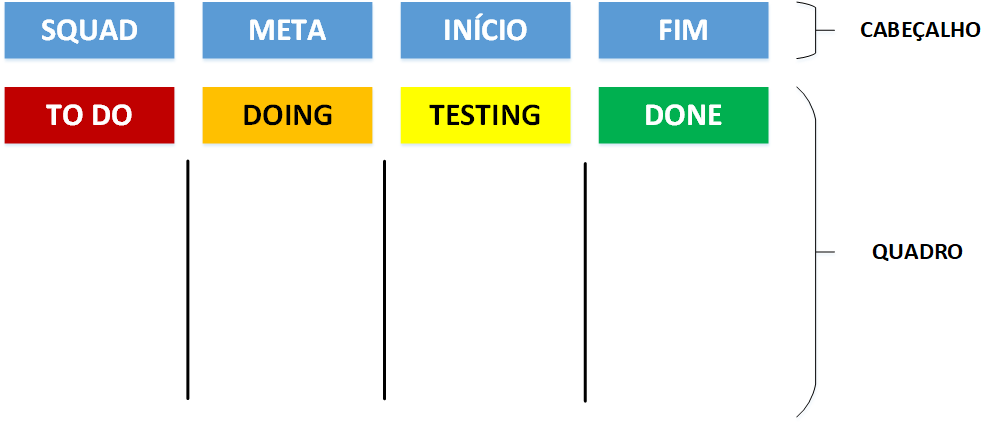
\includegraphics[width=\textwidth]{Kanban}
	\caption{Exemplo de figura do modelo Kanban}
	\label{Kanban}
\end{figure}
Os campos do cabeçalho têm a função de facilitar o acompanhamento da Sprint e uma rápida visualização do progresso do squad, portanto deverão ser especificados no quadro de forma clara mesmo que no caso de um quadro gerenciado em meio virtual. Os campos do cabeçalho são:
\begin{itemize}
	\item \textbf{Squad:} identificação rápida do Squad a quem este quadro pertence (ex: Squad 1, Squad Mobile, Squad API, etc.);
	\item \textbf{Meta:} em alguns casos, nem todos os itens da Sprint poderão ser desenvolvidos, portanto define-se uma meta para considerarmos a Sprint bem-sucedida;
	\item \textbf{Início e Fim:} datas de início e fim planejados da Sprint.
\end{itemize}
As etapas no quadro são:
\begin{itemize}
	\item \textbf{To do:} itens planejados da Sprint que ainda não foram iniciados
	\item \textbf{Doing:} itens que estão em desenvolvimento;
	\item \textbf{Testing:} itens em fase de testes e aprovação;
	\item \textbf{Done:} itens completamente desenvolvidos e devidamente testados.
\end{itemize}

\subsection{Interações}
O processo possui apenas duas principais interações com os Stakeholders do projeto. 

Primeiramente temos uma interação constante entre Line Manager, P.O e Customer, onde são sempre discutidas as demandas do último. É responsabilidade do Line Manager e do P.O a extração de informações das demandas do Customer para a definição dos requisitos, é nessa interação também onde os dois validam as entregas realizadas para verificar se a os requisitos estão sendo atendidos e se novas demandas estão surgindo. 

A segunda interação presente no processo trata-se do alinhamento dos Squads com o Line Manager e Product Owner para um feedback dos Squads, dos membros individualmente e do ciclo como um todo, pontos positivos, pontos negativos, o que se pode aproveitar ou não, coisas novas que foram testadas e demonstraram uma melhoria, ou algo que falhou durante o ciclo. Esta reunião serve como base para um histórico de aperfeiçoamento do processo ao longo das Iterações, a cada ciclo o processo deve ser refinado até atingir os níveis de desempenho desejados, isso não impede que novos métodos sejam testados; 
\subsection{Iterações}
Todo processo é uma iteração. Sendo um ciclo de vida cíclico por completo, o processo repete a fase de levantamento de requisitos até a fase de manutenção quantas vezes forem necessárias até a solução final estiver concluída.


\subsection{Milestones}
Em cada ciclo teremos todas as nossas fases do processo realizadas novamente, deste modo, para que não haja milestones desnecessários ou que possam tornar o processo confuso e/ou lento, foram definidos apenas dois marcos principais em nosso processo. O primeiro se dá ao fato de Definir o Backlog, pois esta tarefa irá definir tudo que será utilizado nas fases e tarefas posteriores, ou seja, com um backlog definido em mãos temos o conteúdo necessário para prosseguir no processo e uma informação para ser comparada com a entrega. 

Quando os itens definidos no backlog passarem pelas fases de desenvolvimento, análise e teste, finalmente poderemos realizar nossa entrega dos artefatos, que é o outro milestone do nosso ciclo. Na entrega temos todo nosso esforço durante o ciclo em forma de conteúdo já validado pela fase de Análise e Teste, provando que o processo foi aplicado de maneira esperada e tal conteúdo entregue atinge os objetivos previamente definidos.
\subsection{Ferramentas}
Os instrumentos recomendados para execução desse processo são:
\begin{itemize}
	\item \textbf{Kanban:} Utilizar algum software que implementa a ideia de Kanban ou post-its para organização das ideias e ciclos.
	\item \textbf{Versionador de Documentos:} Os artefatos gerados durante o ciclo serão atualizados constantemente, é recomendado o uso de algum versionador de documentos como SharePoint; 
	\item \textbf{Versionador de Código:} Todo código-fonte gerado durante o desenvolvimento deve ser versionado para manter um controle de entrega por ciclo, pode ser considerado opções como GIT \cite{git} e SVN \cite{svn}.
\end{itemize}	

\subsection{Feedback}
Feedback é um dos pilares mais importantes propostos no processo descrito neste documento, pois ele deverá caminhar em conjunto com os demais componentes do ciclo de vida para que possamos tomar diferentes posturas e propor melhorias ao processo e aos envolvidos. Dentro desse componente, temos duas vertentes principais, os feedbacks internos e externos em perspectiva ao Squad. 
\begin{itemize}
	\item \textbf{Feedback Interno:} Através dos indicadores gerados a partir dos artefatos o Agile Coach irá propor diferentes posturas dos membros envolvidos no processo e caso necessário realizar pequenas mudanças no processo para o próximo ciclo;
	\item \textbf{Feedback Externo:} O Line Manager obterá informações através de alinhamentos com os Agile Coach’s e acompanhamento do processo e conteúdo desenvolvido dos diferentes Squad’s.  Com os dados obtidos a partir deste controle o Line Manager irá realizar feedbacks coletivos e individuais visando melhorar o desempenho individual dos envolvidos assim como melhorias no processo de cada Squad baseadas nas suas características e ajudará no desenvolvimento da carreira individual dos membros da equipe. 
\end{itemize}	


\section{Ciclo de vida}
Nosso processo foi estruturado de forma que seu ciclo de vida será composto por pequenas iterações que irão englobar todas as fases que serão descritas posteriormente, visando a agilidade nas entregas e melhoria no processo como um todo. Como se trata de um processo ágil, a decisão de que o mesmo seria cíclico foi fundamental, onde teremos constantes revisões nas tarefas ao decorrer de cada ciclo.  

O nascimento do nosso processo caminha em conjunto com as primeiras fases definidas, que envolvem tarefas associadas à planejamento e construção do escopo. Essa etapa de nosso ciclo de vida serve de base para todas etapas seguintes, como à cada ciclo teremos um novo planejamento e uma nova definição do conteúdo a ser trabalhado, o acompanhamento da eficiência desse processo se torna muito mais ágil, pois conseguiremos analisar em pequenas etapas se o processo está sendo efetivo, ou seja, se o conteúdo que está sendo entregue é realmente o que havia sido proposto. 

O fato de todas nossas fases estarem agrupadas de forma cíclica somado à milestones e entregas bem definidas, fazem com que uma possível manutenção no ciclo de vida traga resultados muito mais rápido, já que no ciclo seguinte haverá todo um pensamento no planejamento e quais pontos podem ser ajustados nas demais fases. 

Em certos modelos de processo de software apenas parte do ciclo de vida é cíclica, ou seja, um esforço muito grande pode ser empenhado nas primeiras fases para que só então se inicie uma fase cíclica, como por exemplo, o desenvolvimento.  Uma vantagem do processo proposto nesse documento é uma desativação menos impactante (tempo e custos), pois caso seja necessário a interrupção do processo, apenas o ciclo em andamento será prejudicado, pois todas as entregas produzidas de ciclos anteriores terão suas fases completas, desde a concepção até sua entrega. 

Os benefícios de uma desativação menos agressiva vão além do tempo poupado e menor prejuízo relacionados aos custos. Em cada ciclo temos documentações relacionadas aos artefatos, versionamentos e informação gerada através dos feedbacks. Ou seja, mesmo após um acontecimento inesperado ou negativo, os dados coletados de ciclos prévios irão enriquecer de forma positiva a base histórica da empresa que implementa o processo. 


\section{Métricas e Parâmetros de Monitoramento}



\section{Modelos de Qualidade}

\section{Histórico}


\section{Melhora Contínua}
Com os artefatos gerados durante todo o processo (Relatórios negativos/positivos do ciclo) o Agile Coach analisa esses documentos e tem o objetivo de entender tudo que deu errado analisando o relatório negativo para que não se repeta nos próximos projetos e absorve tudo que foi essencial para conseguir entregar a solução final analisando o relatório positivo. O Line Manager também terá acesso a esses documentos e ao final do projeto ele montará um plano de ação para poder melhorar o processo como um todo, baseado nas experiências anteriores.


\section{BPMN}
\begin{figure}[!htb]
	\centering
	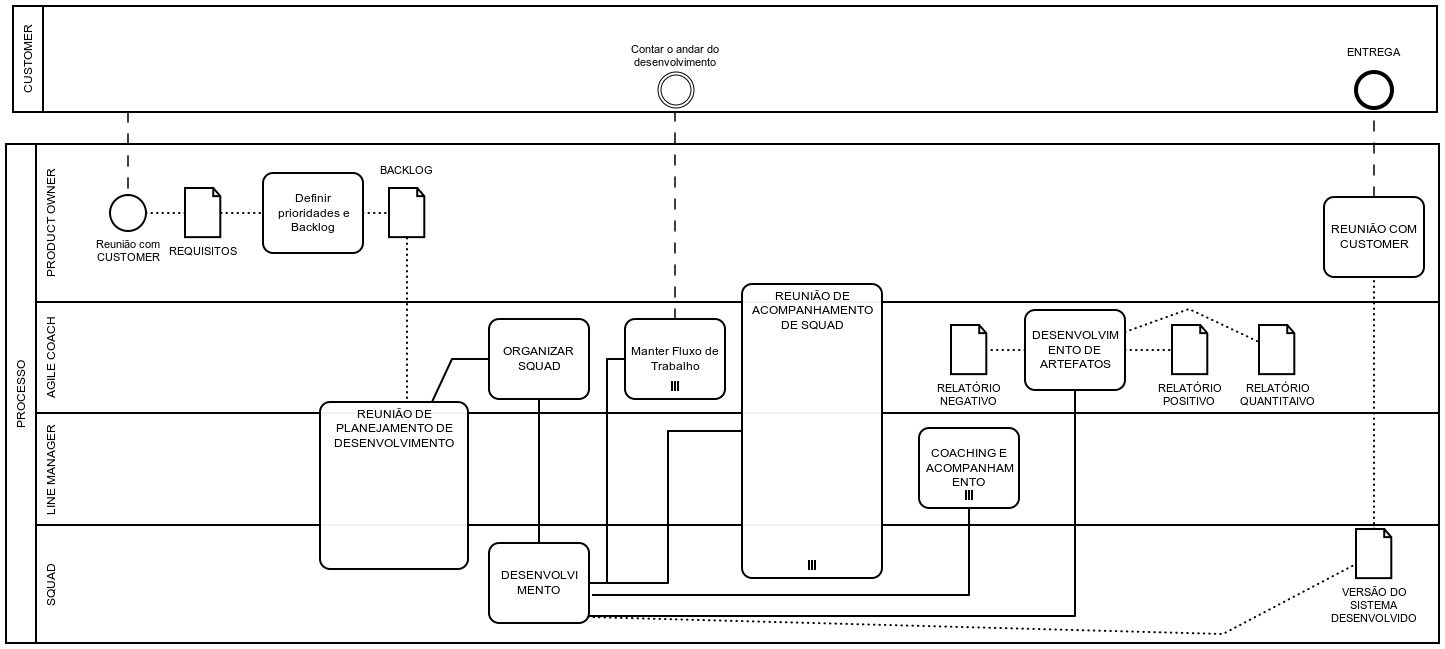
\includegraphics[width=\textwidth]{bpmn}
	\caption{Business Process Model and Notation do Processo BJR}
	\label{bpmn}
\end{figure}

\clearpage
\section{Referências}
\begingroup
\renewcommand{\section}[2]{}

\bibliographystyle{ieeetr}
\bibliography{referencias/referencias} 
\endgroup


\end{document}